%%%%%%%%%%%%%%%%%%%%%%%%%%%%%%%%%%%%%%%%%
% Beamer Presentation
% LaTeX Template
% Version 1.0 (10/11/12)
%
% This template has been downloaded from:
% http://www.LaTeXTemplates.com
%
% License:
% CC BY-NC-SA 3.0 (http://creativecommons.org/licenses/by-nc-sa/3.0/)
%
%%%%%%%%%%%%%%%%%%%%%%%%%%%%%%%%%%%%%%%%%

%----------------------------------------------------------------------------------------
%	PACKAGES AND THEMES
%----------------------------------------------------------------------------------------

\documentclass{beamer}[9pt]

\mode<presentation> {

% The Beamer class comes with a number of default slide themes
% which change the colors and layouts of slides. Below this is a list
% of all the themes, uncomment each in turn to see what they look like.

\usetheme{default}
%usetheme{AnnArbor}
\usetheme{Antibes}
%\usetheme{Bergen}
%\usetheme{Berkeley}
%\usetheme{Berlin}
%\usetheme{Boadilla}
%\usetheme{CambridgeUS}
%\usetheme{Copenhagen}
%\usetheme{Darmstadt}
%\usetheme{Dresden}
%\usetheme{Frankfurt}
%\usetheme{Goettingen}
%\usetheme{Hannover}
%usetheme{Ilmenau}
%\usetheme{JuanLesPins}
%\usetheme{Luebeck}
%\usetheme{Madrid}
%\usetheme{Malmoe}
%\usetheme{Marburg}
%\usetheme{Montpellier}
%\usetheme{PaloAlto}
%\usetheme{Pittsburgh}
%\usetheme{Rochester}
%\usetheme{Singapore}
%\usetheme{Szeged}
%\usetheme{Warsaw}

%\usecolortheme{albatross}
\usecolortheme{beaver}
%\usecolortheme{beetle}
%\usecolortheme{crane}
%\usecolortheme{dolphin}
%\usecolortheme{dove}
%\usecolortheme{fly}
%\usecolortheme{lily}
%\usecolortheme{orchid}
%\usecolortheme{rose}
%\usecolortheme{seagull}
%\usecolortheme{seahorse}
%\usecolortheme{whale}
%\usecolortheme{wolverine}


\setbeamertemplate{footline}[page number] 
\setbeamertemplate{navigation symbols}{}
}

\usepackage{graphicx} % Allows including images
\usepackage{booktabs} % Allows the use of \toprule, \midrule and \bottomrule in tables
\usepackage[utf8]{inputenc}
%----------------------------------------------------------------------------------------
%	TITLE PAGE
%----------------------------------------------------------------------------------------

\title[Reaktorphysik]{Einführung in die Reaktorphysik} 

\author{Martin Bieker}
\subtitle{Kernenergie Seminar WS 14/15}
\date{}

\usepackage{graphicx}
\usepackage{siunitx}
\begin{document}

\begin{frame}
\titlepage 
\end{frame}


\begin{frame}
\frametitle{Überblick}

\begin{columns}[c] 

\column{.4\textwidth} 
\begin{itemize}
\item Kernspaltung
\item Neutronenphysik
\item Vierfaktorformel
\item Der Kritische Reaktor
\end{itemize}

\column{.7\textwidth} 
\begin{figure}[htp]
\centering
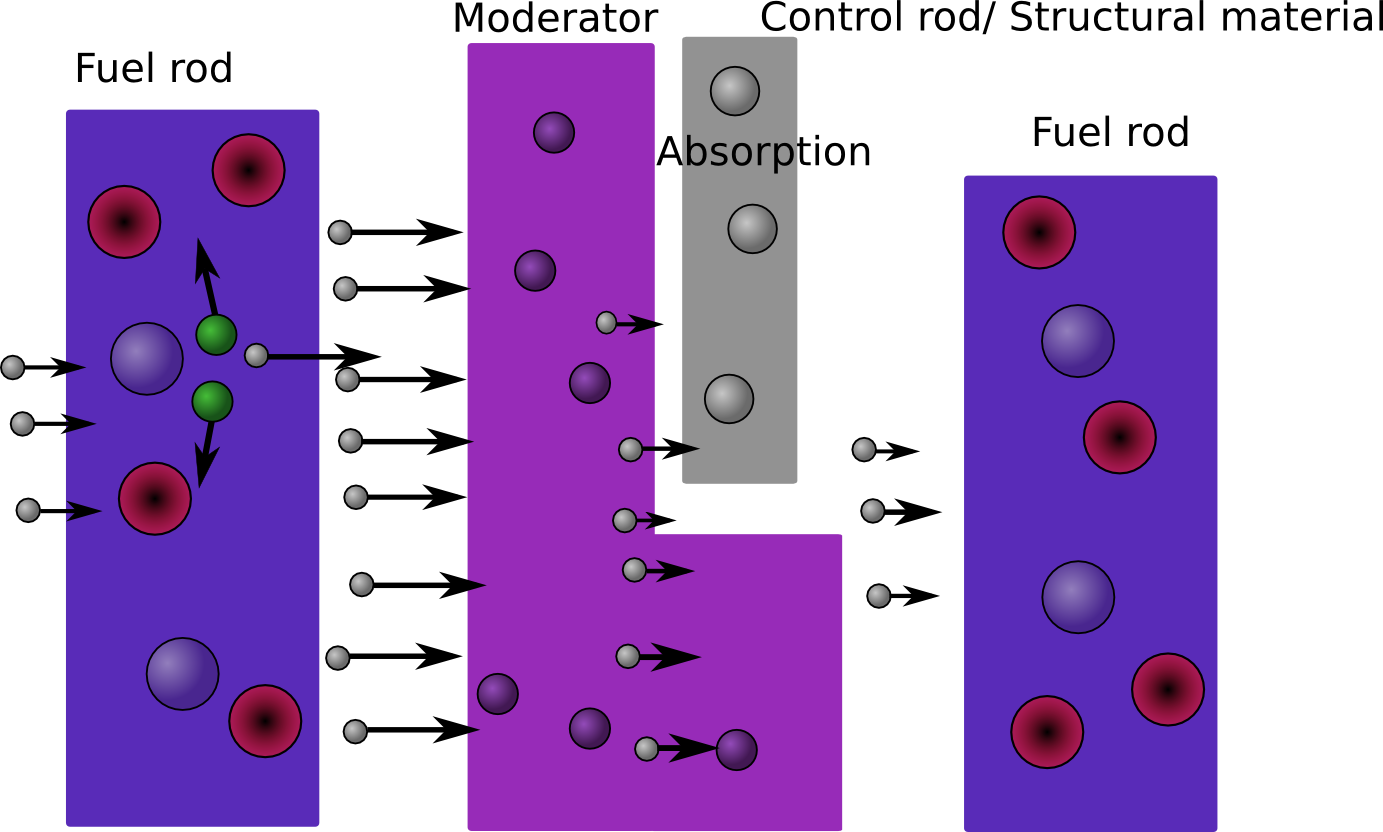
\includegraphics[scale=0.2]{thermal_reactor_full.png}

\end{figure}
\hspace{.5\columnwidth}[1]
\end{columns}


\end{frame}

\section[]{Kernspaltung}

\begin{frame}
\frametitle{Die stoßinduzierte Kernspaltung}

\begin{block}{Die Allgemeine Reaktion}
\[
^{A}_{Z}X + ^1_0n \rightarrow ^{A_1}_{Z_1}Y_1 + ^{A_2}_{Z_2}Y_2 + \nu \cdot ^1_0n
\]

\begin{itemize}
\item$A = A_1 + A_2 + \nu -1 $
\item $Z = Z_1 + Z_2$
\end{itemize}
\end{block}

\begin{block}{Ein Beispiel}
\[
^{235}_{92}U + ^1_0n \rightarrow ^{143}_{56}Ba + ^{90}_{36}Kr + 3 \cdot ^1_0n
\]
\end{block}


\end{frame}



\begin{frame}
\frametitle{Reaktionsenergie der Kernspaltung}

\begin{block}{Erinnerung: Weizsäcker Massenformel \& Masse Energie Äquivalenz}
\[
m(Z,A) = Z \cdot m_p + (A-Z)\cdot m_n - \frac{E_B}{c^2}
\]
\[
E = mc^2
\]
\end{block}

Für die Reaktionsenergie einer Kernreaktion gilt:
\[
E_f = \Delta m \cdot c^2
\]
mit dem Massendefekt:
\[
\Delta m = m(\mathrm {Edukte})-m(\mathrm{Produkte})
\]
\end{frame}

\begin{frame}
\frametitle{Massenbilanz der Kernspaltung}

\centering
\begin{columns}
\centering
\column{0.4\textwidth}


\textbf{Vor der Reaktion}

\vspace*{0.5cm}
\begin{tabular}{lr}
\toprule
	Teilchen & $\frac{Masse}{\si{\giga\eV}}$ \\
\midrule	
	Uran-235 & \num{218.887}\\
	\\
	Neutron & \num{.940}\\
	\midrule
	Gesamt & 219.827\\
	\bottomrule
	
\end{tabular}
\column{0.4\textwidth}

\centering
\textbf{Nach der Reaktion}

\vspace*{0.5cm}
\begin{tabular}{lr}
\toprule
	Teilchen & $\frac{Masse}{MeV}$ \\
\midrule	
	Barium-143 & \num{133.072}\\
	Krypton-90 & \num{83.740}\\
	3 Neutronen & $3 \cdot\num{.940}$\\ 
	\midrule
	Gesamt & \num{219.632}\\
	\bottomrule
\end{tabular}
\end{columns}
\vspace{0.5cm}
\[
E_f = \Delta m = \SI{195}{\MeV} \approx  \SI{200}{\MeV} 
\]
\end{frame}

\begin{frame}
\frametitle{Kernenergie vs. "Atomenergie"}
\framesubtitle{Energiedichten von Uran im Vergleich zu konventionellen Energieträgern}
\begin{columns}
\column{.55\textwidth}
\begin{itemize}
\item Berechnung der Energiedichte:
\[
w = E_f \cdot \frac{ N_A }{M_{U-235}} = \SI{8.81e13}{\joule\per\kilogram}
\]
\item Vergleich mit konventionellen Energieträgern:\\

\begin{description}

\item[ Kohle:] \SI{2.88e4}{\joule\per\kg}
\item[Erdöl:] \SI{3.96e4}{\joule\per\kg}

\end{description}
\end{itemize}
\column{.5\textwidth}
\begin{figure}[htp]
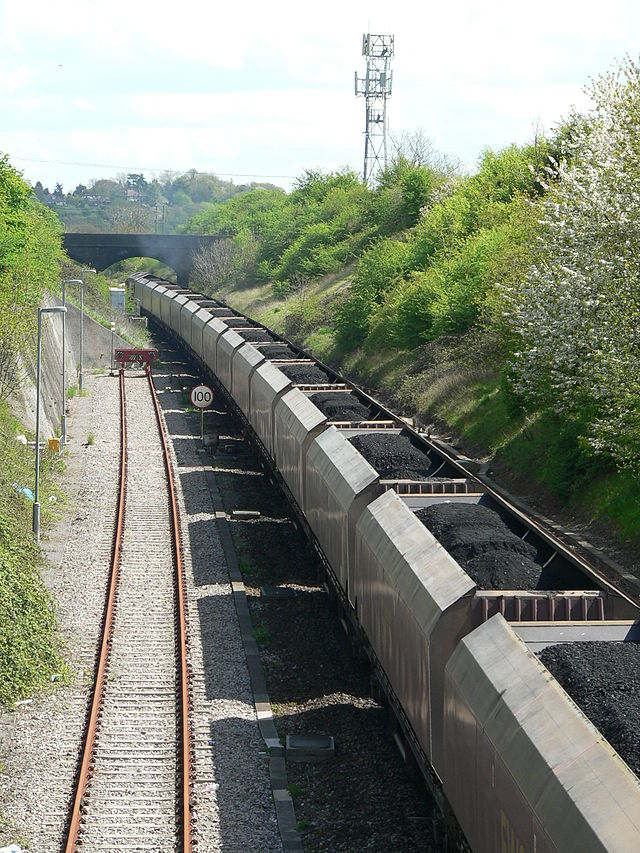
\includegraphics[scale=.15]{coal.jpg}
\end{figure}
\hspace{.5\columnwidth}[2]
\end{columns}
\end{frame}



\begin{frame}
\begin{columns}
\frametitle{Spaltstoffe}
\framesubtitle{Übersicht über verschiedene Spaltstoffe}
\column{0.55\textwidth}

Natürliche Spaltstoffe:
\begin{itemize}
\item Uran-235 (0.7 \% in natürlichem Uran)
\end{itemize}
Erbrütete Spaltstoffe:
\begin{itemize}
\item Plutonium-239
\item Plutonium-241
\item Uran-233

\end{itemize}
\column{0.45\textwidth}
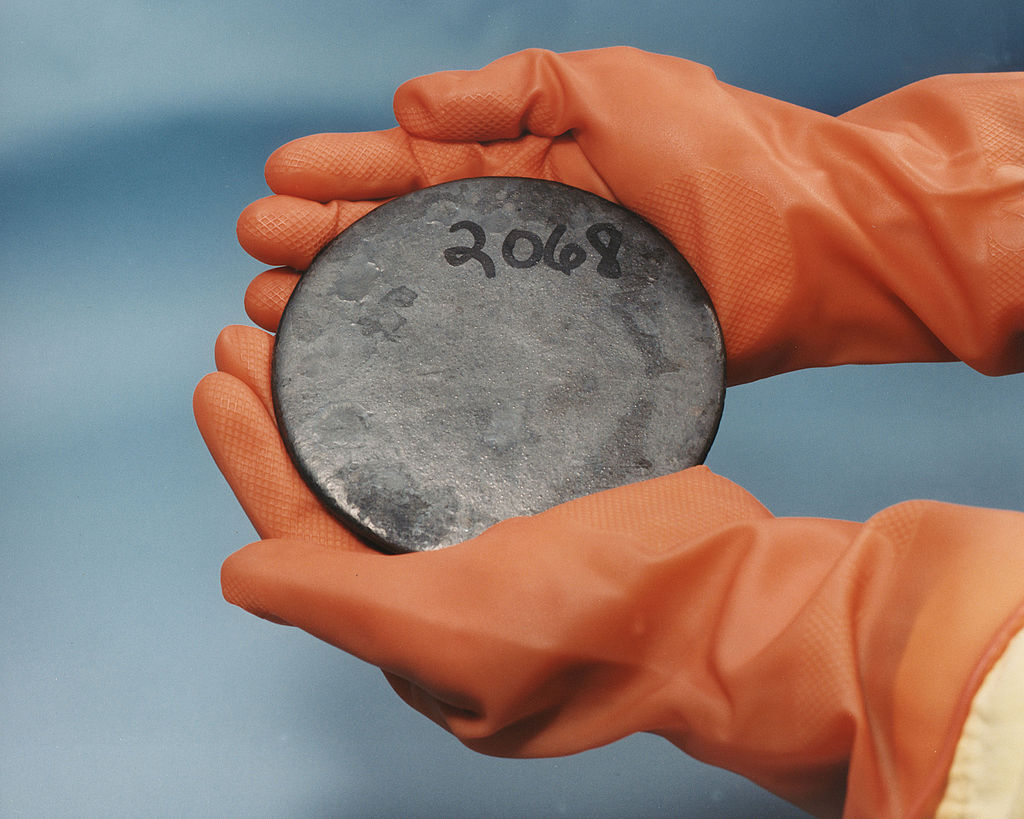
\includegraphics[scale=0.55]{HEUranium.jpg}\\
\textit{Hochangereichertes Uranmetall (99 \% U-235)} [3]
\end{columns}
\vspace{1em}
Die Brutstoffe werden durch Kernreaktionen im Reaktor erzeugt.
\end{frame}

\begin{frame}
\frametitle{Spaltprodukte}
\begin{columns}

\column{.4\textwidth}
\begin{itemize}

\item Bei der Kernspaltung entstehen zwei Tochterkerne
\item Diese sind meist instabil und zerfallen weiter.
\item Auch nach Abschalten der Kettenreaktion entsteht Nachzerfallswärme
\item[$\rightarrow$] Diese muss sicher abgeführt werden
\end{itemize}
\column{.6\textwidth}
\begin{figure}

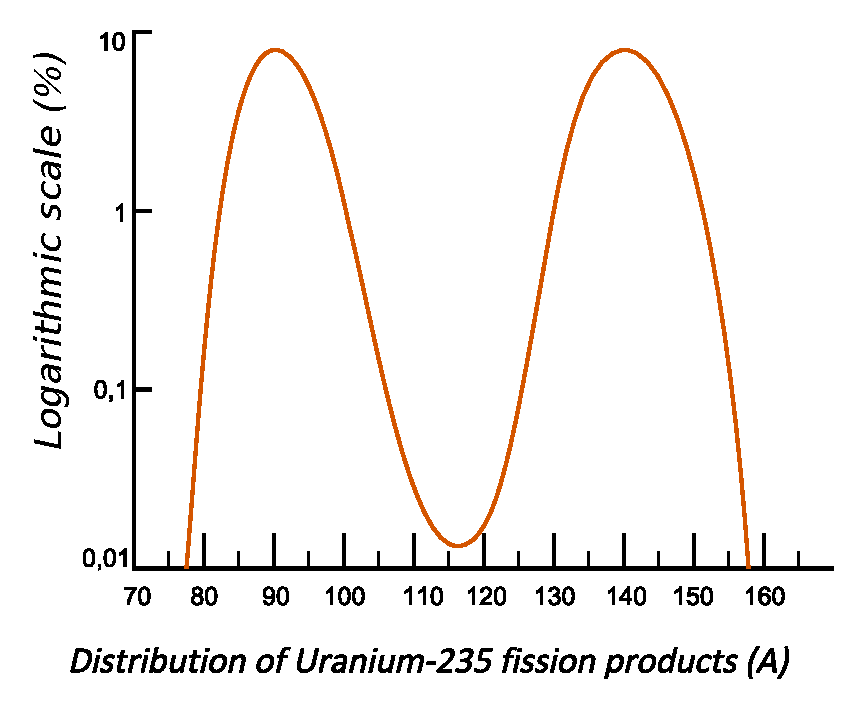
\includegraphics[scale=.45]{fission_products.pdf}
\end{figure}
\hspace{.5\columnwidth}[4]
\end{columns}
\end{frame}

\begin{frame}
\frametitle{Spaltprodukte}
\framesubtitle{Zerfallsketten}
\begin{columns}
\column{.5\textwidth}
\begin{figure}
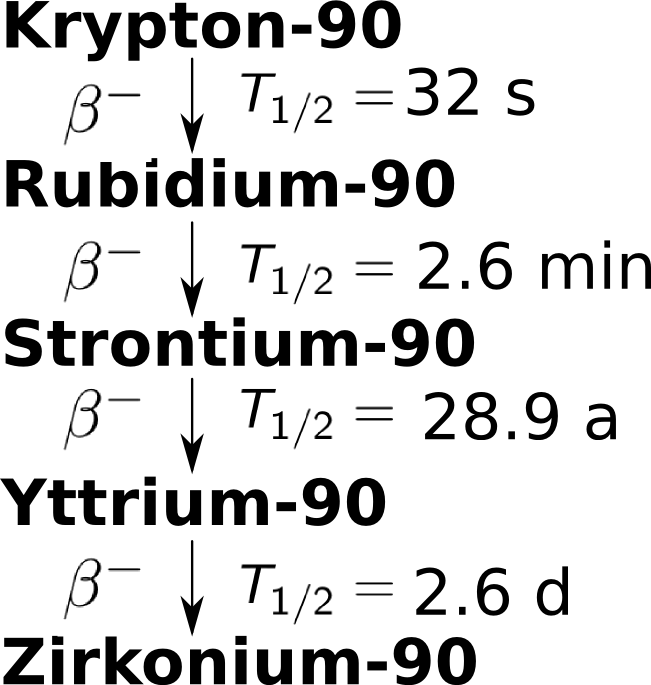
\includegraphics[scale=.2]{zerfallsreihe.png}
\end{figure}

\column{.5\textwidth}
\begin{figure}
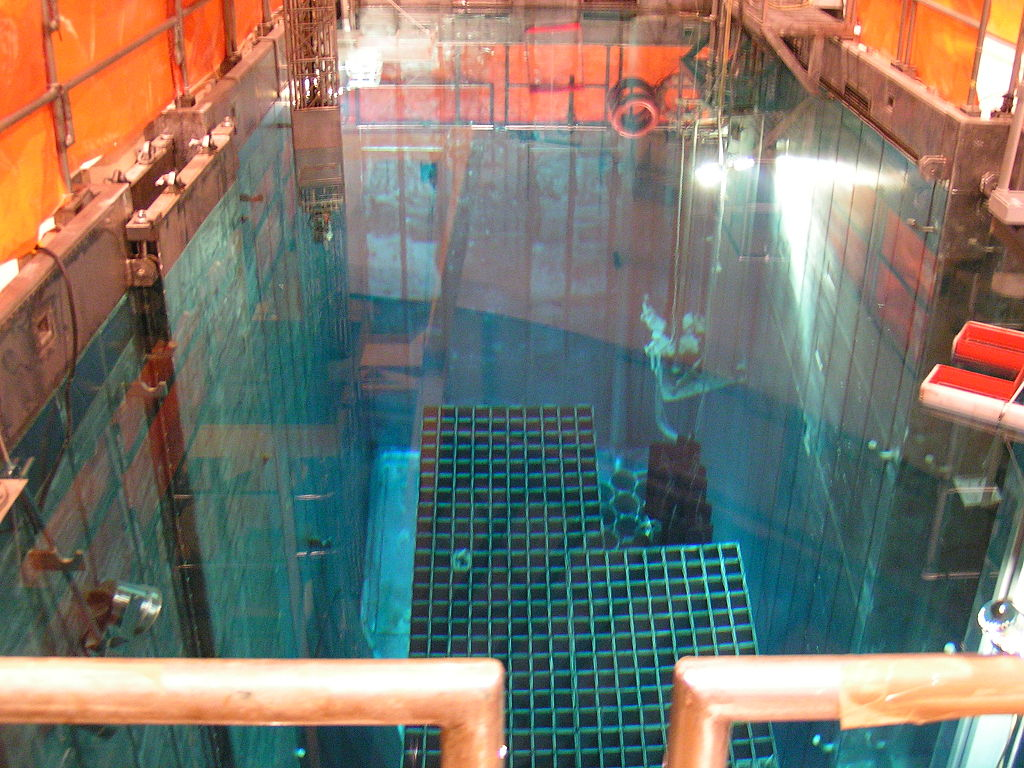
\includegraphics[scale=.15]{abklingbecken.jpg}
\end{figure}
\hspace{.5\columnwidth}[5]
\end{columns}
\end{frame}


\begin{frame}
\frametitle{Neutronenemission}
\framesubtitle{prompt und verzögert}
\begin{itemize}
\item Neutronen werden mit einer Energie von durchschnittlich $\SI{2}{\MeV}$ emittiert (schnelle Neutronen).
\item $\SI{99.35}{\percent}$ aller Neutronen werden spontan (prompt) abgegeben.
\item Diese entstehen innerhalb von $\SI{1e-4}{\second}$   nach der Kernspaltung.
\item Die restlichen Neutronen entstehen durch Zerfälle der Spaltprodukte.
\item Dies geschieht Sekunden bis Minuten nach der Kernspaltung
\item Verzögerte Neutronen sind für die Reaktorsteuerung unverzichtbar.
\end{itemize}
\end{frame}




\begin{frame}
\frametitle{Neutronenfluss und Wirkungsquerschnitt}
\begin{block}{Neutronenflussdichte}
\begin{description}
\item[Energieabhängig:]$\Phi(E,\vec r) = \vec v(E,\vec r)\cdot \rho_n(E,\vec r)$
\item[Gesamtflussdichte:] $\Phi_{ges}(\vec r)= \int_0^{E_{max}}\Phi(E, \vec r) dE$
\end{description}

\end{block}

\begin{block}{Makroskopischer Wirkungsquerschnitt}
\[
\Sigma = \sigma \cdot N = \frac{m\cdot N_A}{M}\cdot \sigma
\]
\end{block}
\end{frame}

\begin{frame}
\frametitle{Reaktionsraten und Reaktorleistung}



\begin{block}{Reaktionsrate}
\[
R = \Phi \cdot \sigma \cdot \rho_N = \Phi \cdot \Sigma 
\]
\begin{description}
\item[$\Phi$:] Neutronenfluss
\item[$\sigma$:] mikroskopischer Wirkungsquerschnitt
\item[$\rho_N$:] Targetdichte

\end{description}
\end{block}

\begin{block}{Reaktorleistung}
\[
P = E_f \cdot R = R \cdot \Phi \cdot \Sigma
\]
\end{block}

\end{frame}

\begin{frame}
\frametitle{Energiespektren von Neutronen}
\begin{itemize}
\item Viele Wechselwirkungen von Neutronen sind stark energieabhängig.
\item Neutronen werden nach Energie unterschieden:
\begin{description}[(schnelle) Spaltneutronen:]
\item[(schnelle) Spaltneutronen:] $ \SI{10}{\kilo\eV}< E < \SI{20}{\mega\eV}$
\item[mittelschnelle Neutronen:] $\SI{0.5}{\eV}< E <\SI{10}{\kilo\eV}$
\item[epithermische Neutronen:]$E < \SI{1}{\eV}$ 
\item[thermische Neutronen:] $E <\SI{ 100}{\milli\eV}$
\end{description}
\end{itemize}
\end{frame}



\begin{frame}
\frametitle{Wechselwirkungen von Neutronen}
Neutronen wechselwirken mit der Materie im Reaktor auf verschiedene Arten:
\begin{itemize}
\item (stoßinduzierte) Kernspaltung
\item Streuung (elastisch / inelastisch)
\item $X + ^1_0n \rightarrow Y + 2\cdot ^1_0n$ 
\item  $X + ^1_0n \rightarrow Y + ^4_2\alpha$  \picture(0,0)\put(5,-9){$\left.\rule{0pt}{3ex}\right\}$ Parasitäre Absorption}\endpicture
\item  $X + ^1_0n \rightarrow Y +\gamma$

\end{itemize}
\end{frame}



\begin{frame}
\frametitle{Kernspaltung}
\framesubtitle{Wirkungsquerschnitt}
\begin{columns}
\column{.4\textwidth}
\begin{itemize}
\item Kernspaltung läuft bei niedrigen Energien (Thermische Neutronen) ab.
\item Neutronen, die bei Kernspaltungen enstehen, haben Energien von $\SI{}{\eV}$.
\item [$\rightarrow$] Moderator benötigt
\end{itemize}
\column{.6\textwidth}
\begin{center}
\vspace{-.6cm}
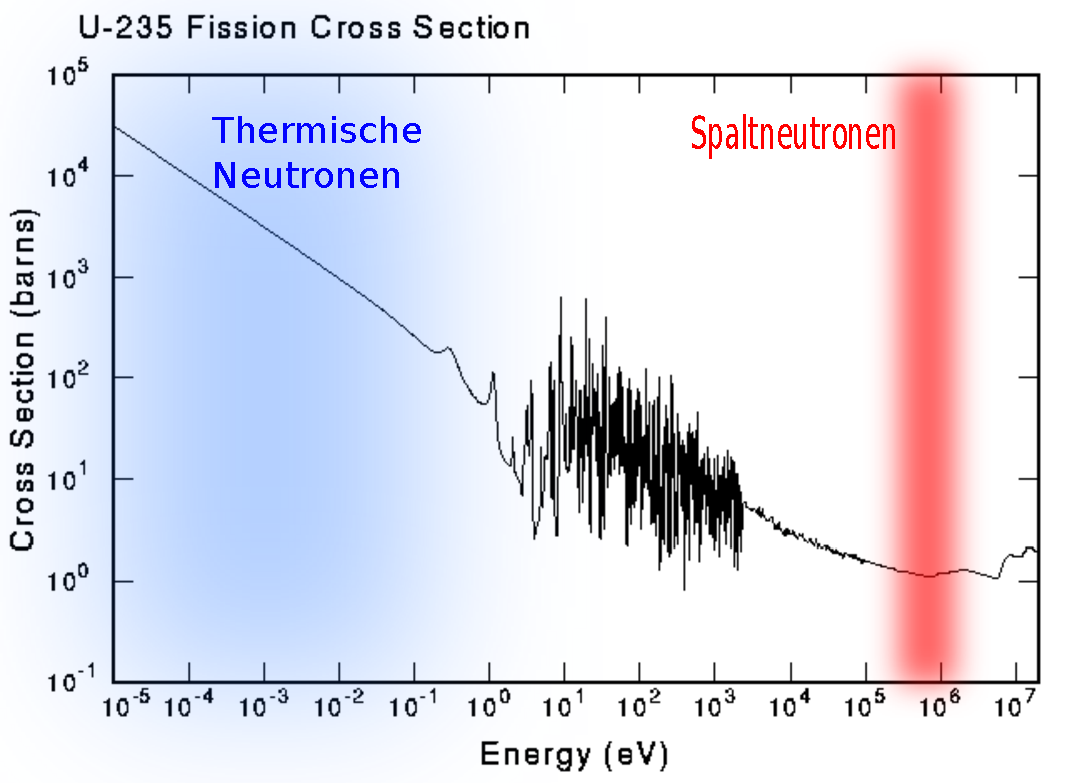
\includegraphics[scale=0.35]{u235_fission_cs.pdf}

\textit{Spaltquerschnitt von U-235 in Abhängigkeit von der Neutronenenergie} [6]

\end{center}
\end{columns}
\end{frame}


\begin{frame}
\frametitle{Absorption von Neutronen}
\begin{columns}
\column{.60\textwidth}
\begin{itemize}
\item Beispiele:

\item[B:] $^{10}_5B + ^1_0n \rightarrow ^{7}_3Li + ^4_2\alpha$
\vspace{0.2cm}
\item[Cd:] $^{113}_{48}Cd + ^1_0n \rightarrow ^{114}_{48}Cd + \gamma$

\vspace{0.2cm}
\item Bei niedrigen Neutronenenergien: $\sigma(E) \propto  \frac{1}{\sqrt{E}}$
\item Stark erhöhter Wirkungquerschnitt im Resonanzbereich
\item Wichtig für die Steuerung des Reaktors $\rightarrow$ Steuerstäbe
\end{itemize}

\column{.4 \textwidth}
\vspace{-1.2cm}
\begin{figure}
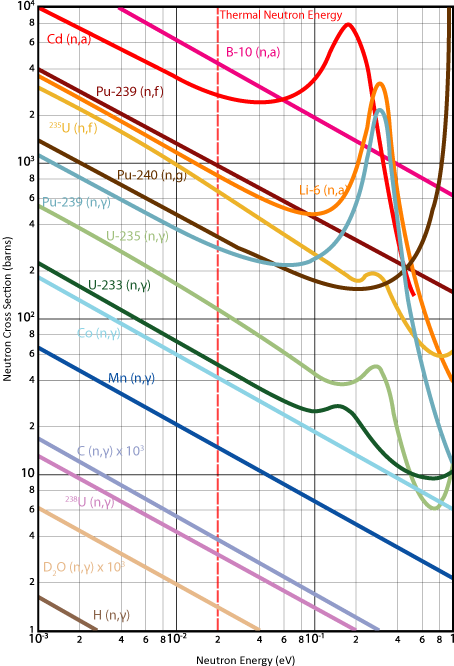
\includegraphics[scale=0.25]{multi_absorption_cs.jpg}\\
\textit{Wirkungsquerschnitte für verschiedene Reaktormaterialien} [7]
\end{figure}
\end{columns}
\end{frame}




\begin{frame}
\frametitle{Absorption von Neutronen}
\framesubtitle{Wirkungsquerschnitt für U-238}
\begin{columns}

\column{.35\textwidth}
\begin{itemize}
\item Niedrig angereichertes Uran besteht zu $\SI{97}{\percent}$ aus U-238.
\item Abgebremste Spaltneutronen durchqueren den Resonanzbereich.
\item [$\rightarrow$] Signifikante Neutronenverluste durch Resonanz
\end{itemize}


\column{.65\textwidth}
\begin{figure}
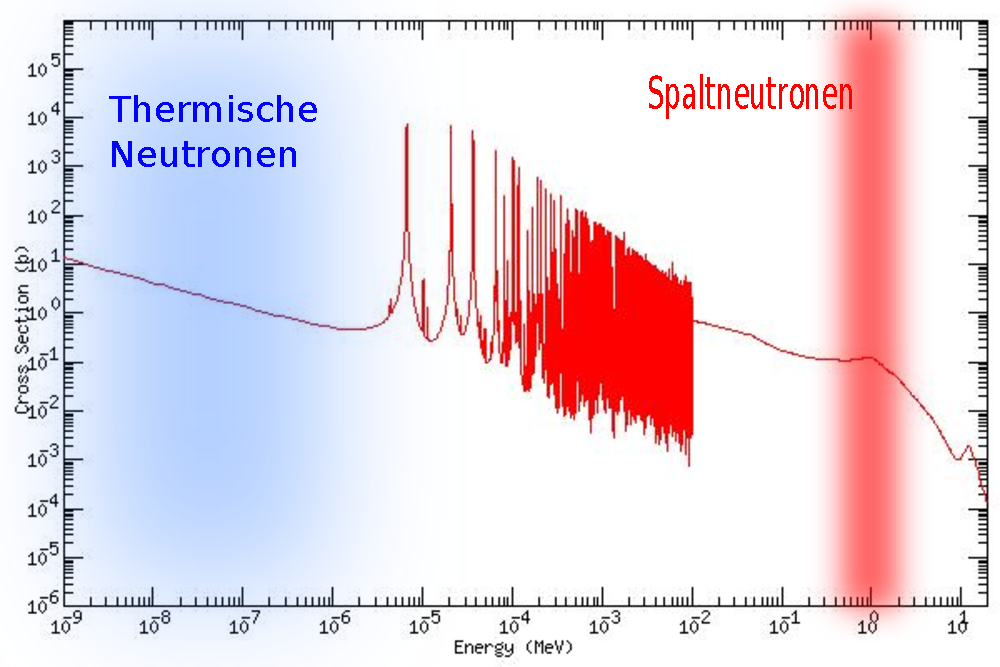
\includegraphics[scale=0.3]{u238_absorption_cs.pdf}
\end{figure}
\hspace{.5\columnwidth}[8]
\end{columns}
\end{frame}




\begin{frame}
\frametitle{Moderation}
\begin{itemize}
\item Spaltneutronen haben Energien im $\si{\mega\eV}$ Bereich.
\item Zum Erreichen günstiger Spaltquerschnitte müssen die Neutronen abgebremst werden.
\item Dazu werden im Reaktor Moderatoren verwendet.
\item Beispiele

\begin{itemize}
\item Wasser
\item Graphit
\end{itemize}

\item Abbremsung erfolgt vor Allem durch:
\begin{itemize}
\item[$\rightarrow$] elastische Stöße

\end{itemize}
\item Diese Vorgänge lassen sich mit klassischer Mechanik modellieren.
\end{itemize}

\end{frame}


\begin{frame}
\frametitle{Moderation}
\framesubtitle{Wichtige Größen}



\begin{columns}
\column{.7 \textwidth}
\begin{itemize}
\item Der relative Energieverlust pro Stoß ist konstant.
\item Neue Größe $\rightarrow$ Lethargie:\\
\vspace{0.5em}
$
u = \ln{\frac {E_0}{ E}}
$
\item Mittlerer Lethargiegewinn pro Stoß:\\
\vspace{0.5em}
$
\xi =1- \frac{(A-1)^2}{A} \cdot \ln{\frac{A+1}{A-1}}
$

\end{itemize}
\column{.3 \textwidth}
\begin{figure}

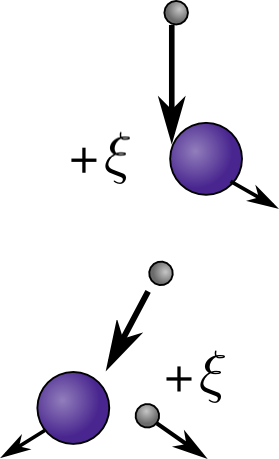
\includegraphics[scale=.3]{moderator.png}

\end{figure}

\end{columns}

\begin{columns}
\column{.7 \textwidth}
\begin{itemize}

\item Anzahl der Stöße zum Abbremsen auf thermische Energien:\\\vspace{0.5em}
$
z = \frac{1}{\xi}\ln{\frac{E_0}{E_{th}}}
$
\end{itemize}
\column{.3 \textwidth}
\hspace{.5\columnwidth}[9]
\end{columns}
\end{frame}


\begin{frame}
\frametitle{Kettenreaktion}
\framesubtitle{Kriterium für Stabilität}

\begin{itemize}
\item Reaktorsteuerung ist unabdingbar für die zivile Nutzung der Kernenergie
\begin{itemize}
\item[$\rightarrow$] kontrollierte Kernspaltung
\end{itemize}
\item Es muss für eine ausgeglichene Neutronenbilanz gesorgt werden.

\begin{eqnarray*}
\frac{d \rho_n}{dt}& =& \nu\cdot \Sigma_f \cdot \Phi - \Sigma_f \cdot \Phi  - \Sigma_a\cdot\Phi\\& = & \rho_n\cdot v \cdot \left[\left(\nu - 1 \right)\Sigma_f - \Sigma_a
 \right]\\&=& C\cdot \rho_n
\end{eqnarray*}
\end{itemize}
\end{frame}


\begin{frame}
\frametitle{Kettenreaktion}
\framesubtitle{Kriterium für Stabilität}

Fallunterscheidung:
\begin{description}
\item[$C > 0$:] überkritischer Reaktor
\item[$C < 0$:] unterkritischer Reaktor
\item[$C = 0$:] kritischer Reaktor
\begin{block}{Multiplikationsfaktor }

\[
 k = \frac{C}{\Sigma_a}+1 =  \sigma_f\cdot\frac{\nu-1}{\Sigma_a}
\]
Für $k=1$ ist der Reaktor \textit{kritisch}.
\end{block} 
\end{description}
\end{frame}


\begin{frame}
\frametitle{Vierfaktorformel}
\framesubtitle{Herleitung für unendliche Reaktoren}
\begin{itemize}
\item unendlicher Reaktor $\rightarrow$ kein Neutronenverlust nach außen.
\end{itemize}

\begin{figure}
\centering
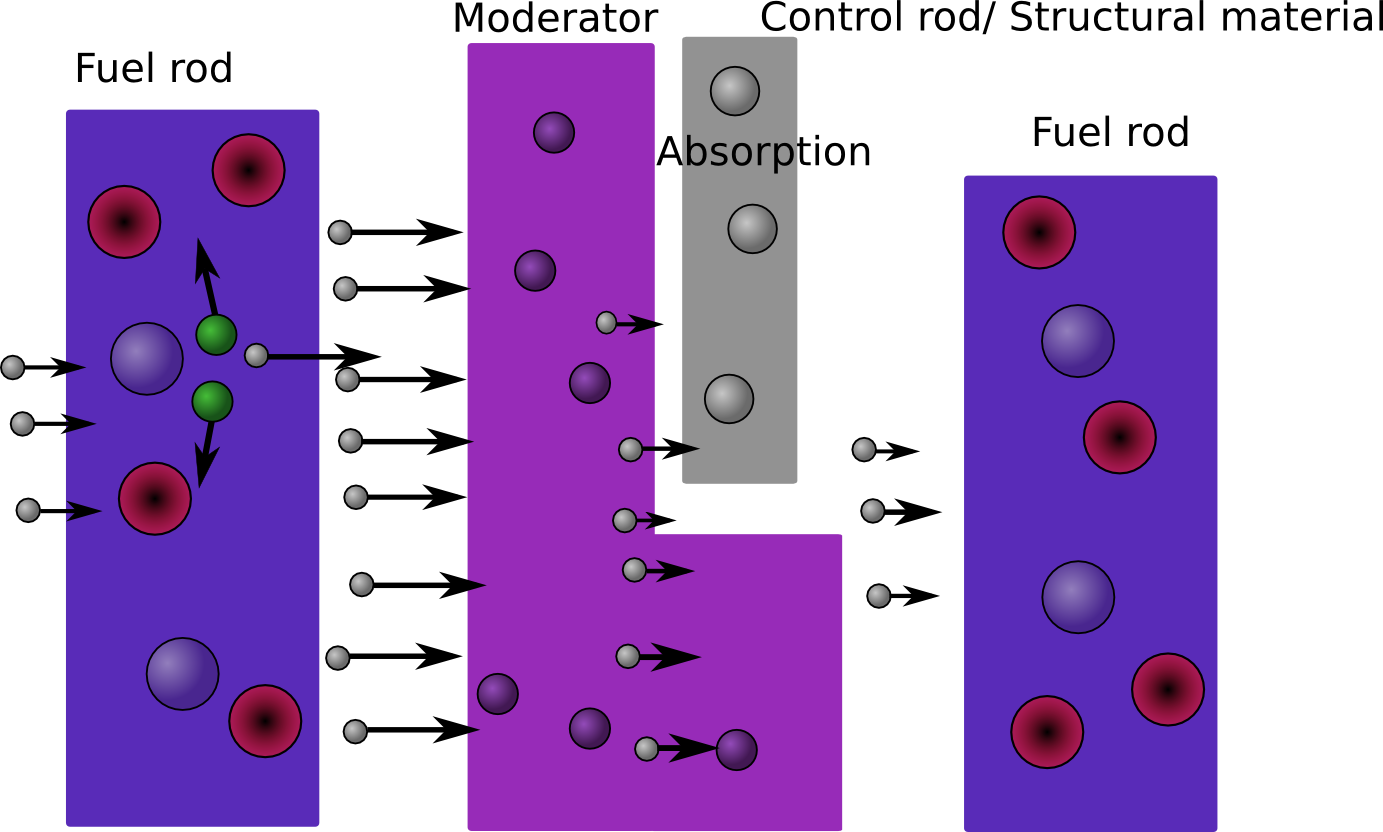
\includegraphics[scale=.2]{thermal_reactor_full.png}
\end{figure}
\hspace{.5\textwidth}[10]
\end{frame}


\begin{frame}
\frametitle{Vierfaktorformel}
\framesubtitle{Herleitung für unendliche Reaktoren}
\begin{itemize}
\item Beginn mit $n$ thermischen Neutronen.
\item Die Neutronen werden im Brennstoff absorbiert.
\item[]
\item[]
\end{itemize}

\begin{figure}
\centering
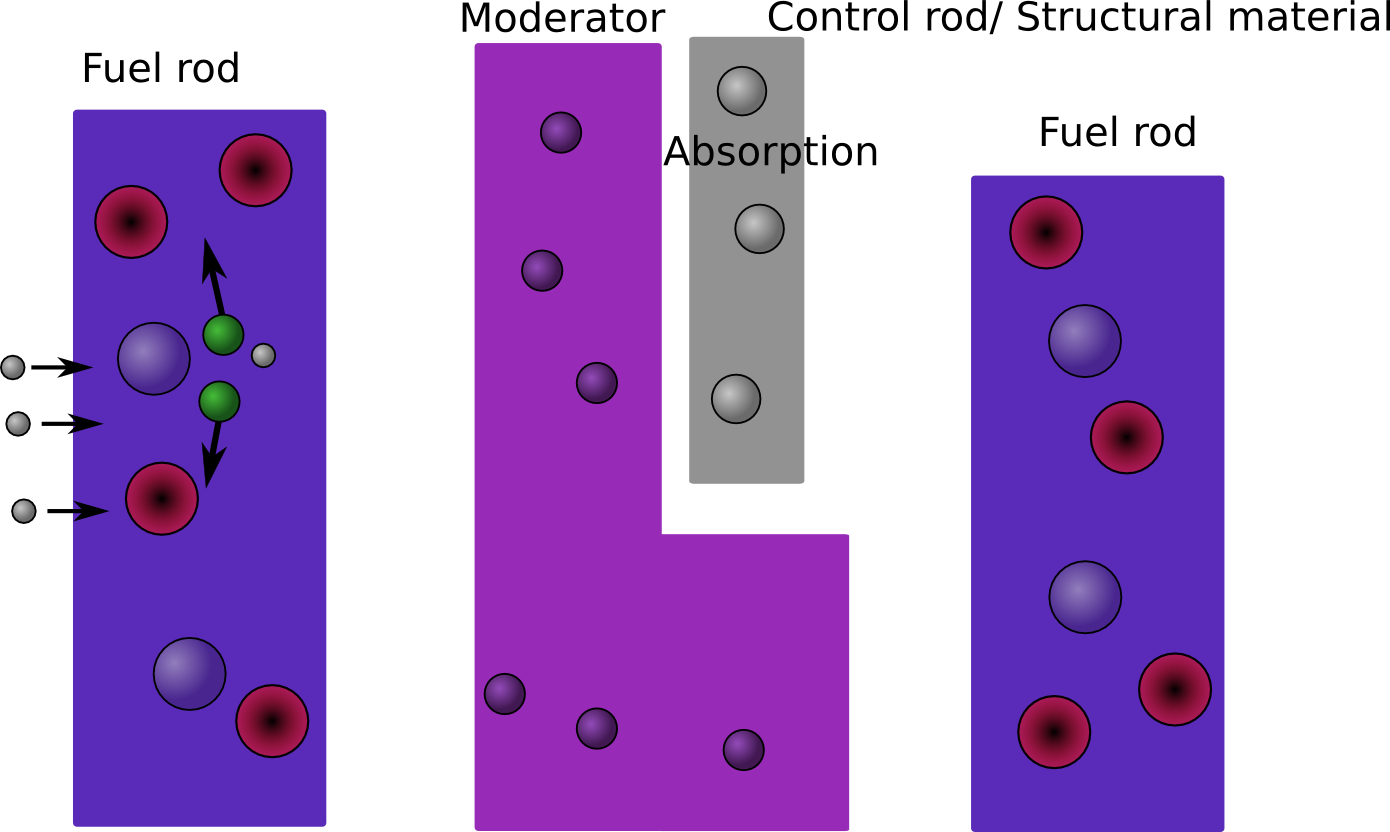
\includegraphics[scale=.15]{thermal_reactor_1.png}[10]
\end{figure}

\end{frame}


\begin{frame}
\frametitle{Vierfaktorformel}
\framesubtitle{Herleitung für unendliche Reaktoren}
\begin{itemize}
\item Es enstehen $n\cdot\eta$ schnelle Spaltneutronen.
\item Durch schnelle Spaltung entstehen $n\cdot\eta\cdot\epsilon$ Neutronen.
\item[$\eta$ :]Neutronenausbeute
\item[$\epsilon$ :]Schnellspaltfaktor
\end{itemize}

\begin{figure}
\centering
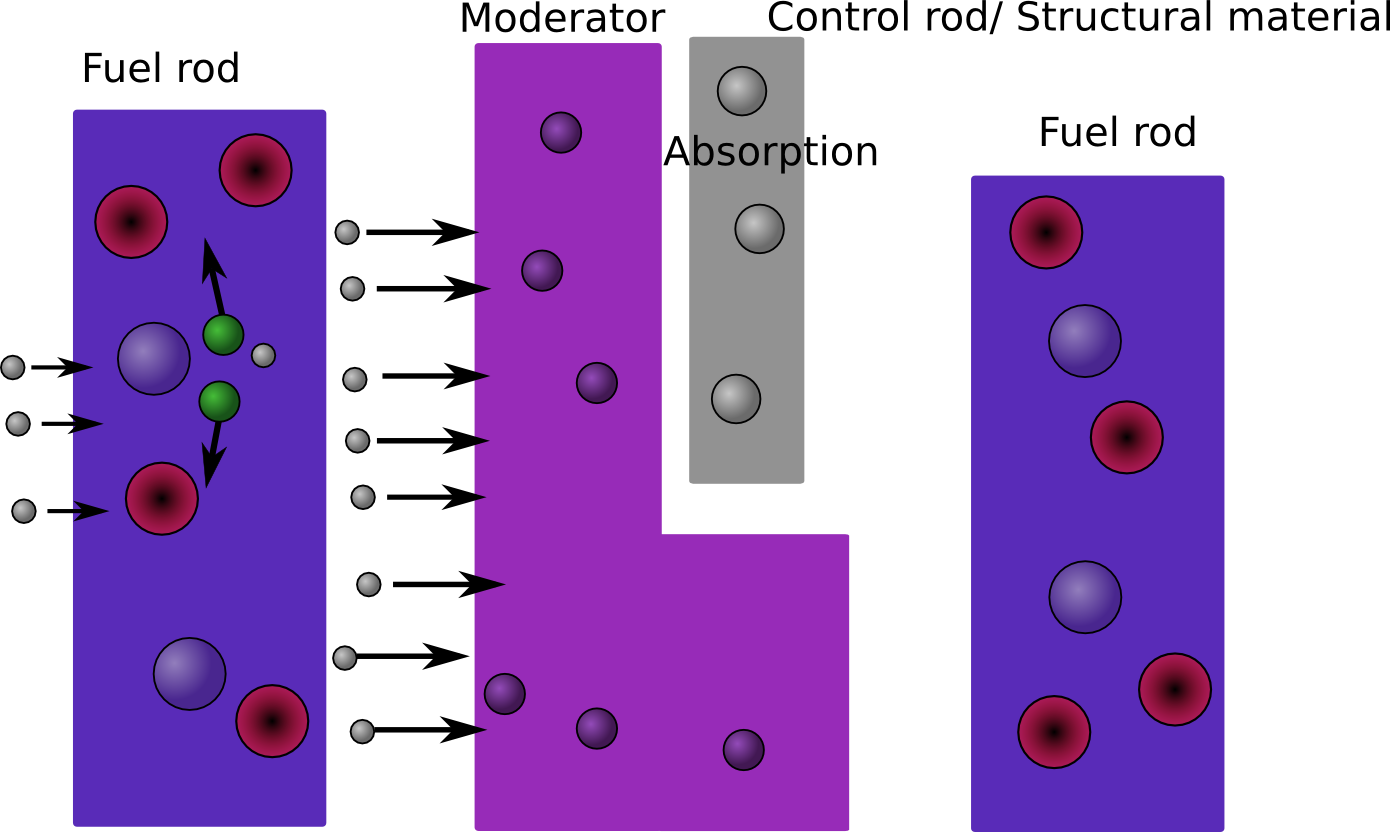
\includegraphics[scale=.15]{thermal_reactor_2.png}[10]
\end{figure}
\end{frame}


\begin{frame}
\frametitle{Vierfaktorformel}
\framesubtitle{Herleitung für unendliche Reaktoren}
\begin{itemize}
\item Neutronen werden im Moderator abgebremst.
\item Dabei durchlaufen sie den Resonanzbereich des U-238
\item Nach der Moderation sind $n\cdot\eta\cdot\epsilon\cdot p $  thermische
 Neutronen vorhanden.\\
 \item[p: ] Resonanzentkommwahrscheinlichkeit 
\end{itemize}

\begin{figure}
\centering
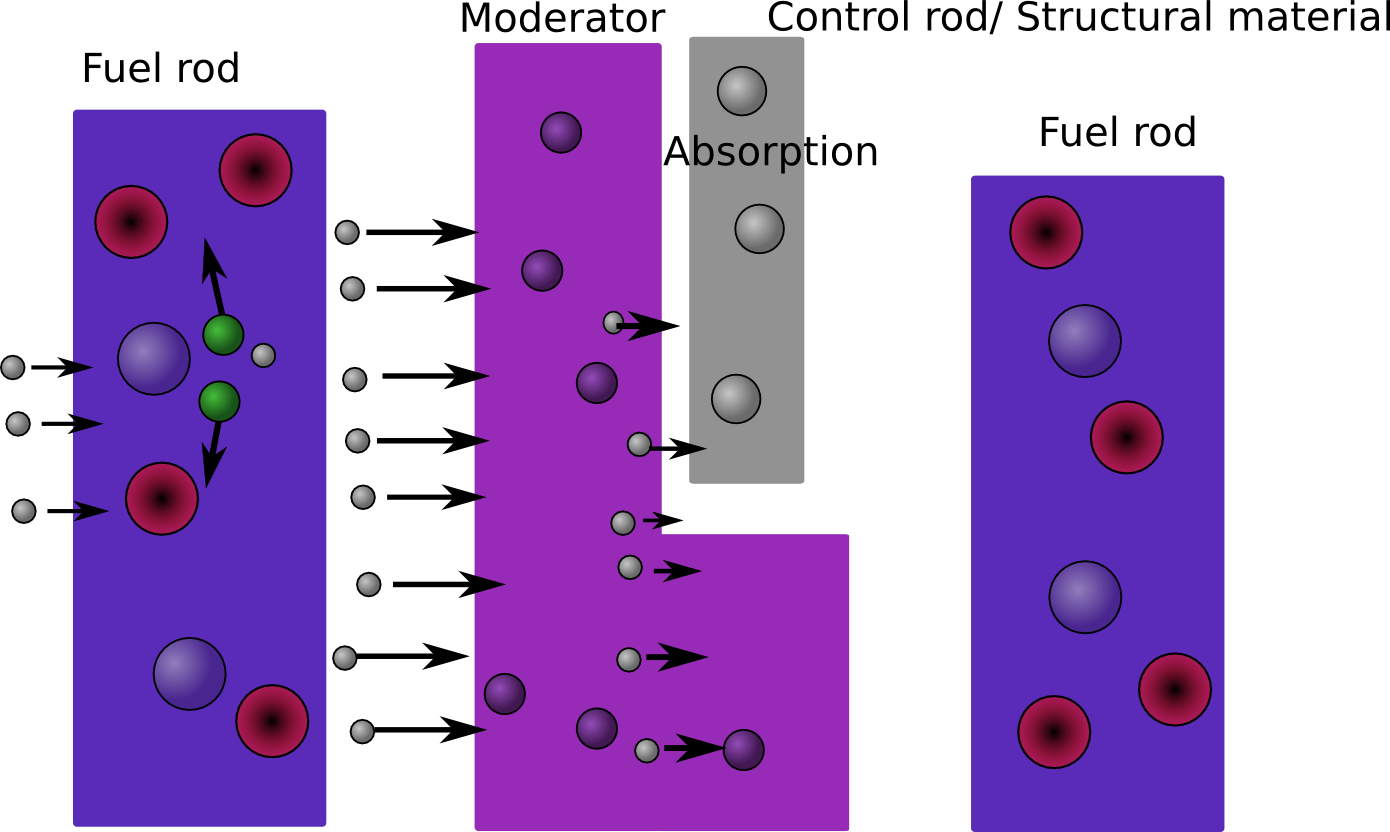
\includegraphics[scale=.15]{thermal_reactor_3.png}[10]
\end{figure}

\end{frame}


\begin{frame}
\frametitle{Vierfaktorformel}
\framesubtitle{Herleitung für unendliche Reaktoren}
\begin{itemize}
\item Ein Teil der Thermischen Neutronen werden im Moderator oder in Strukturmaterialien absorbiert.
\item Es stehen  $n\cdot\eta\cdot\epsilon\cdot p\cdot f$ Neutronen für weitere Kernspaltungen zur Verfügung.
\item[f: ]Thermische Nutzung
\end{itemize}

\begin{figure}
\centering
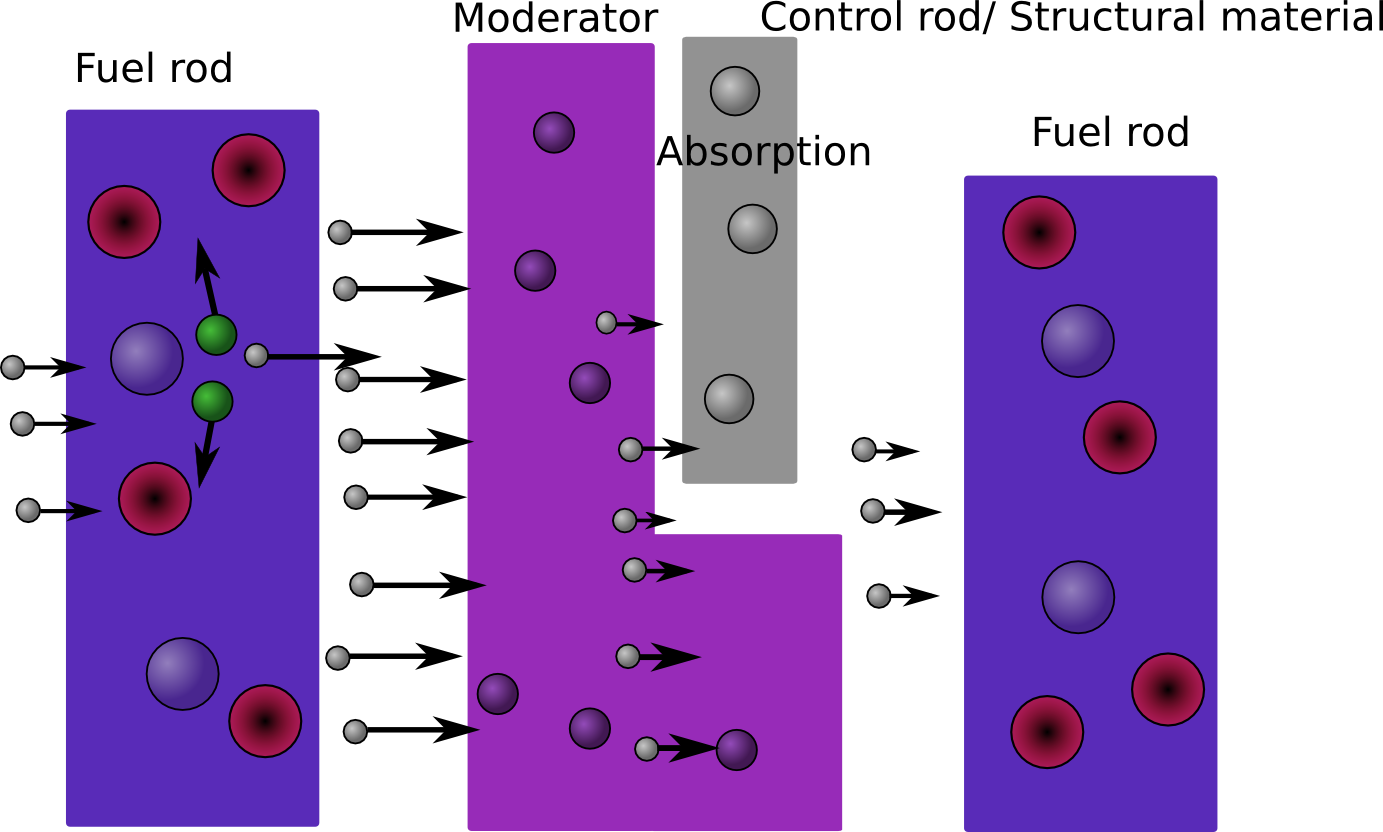
\includegraphics[scale=.15]{thermal_reactor_full.png}[10]
\end{figure}
\end{frame}

\begin{frame}
\frametitle{Vierfaktorformel}
\framesubtitle{Zusammenfassung für unendliche Reaktoren}
Für eine stabile Kettenreaktion muss gelten:
\[
n = n\cdot\eta\cdot\epsilon\cdot p\cdot f \Leftrightarrow 1 = \eta\cdot\epsilon\cdot p\cdot f 
\]
Es ergibt sich die
\begin{block}{Vierfaktorformel für unendliche Reaktoren}
\[
k_\infty =  \eta\cdot\epsilon\cdot p\cdot f
\]
\begin{description}
\item[$\eta$:] Neutronenausbeute
\item[$\epsilon$:] Schnellspaltfaktor
\item[$p$:] Resonanzentkommwahrscheinlichkeit
\item[$f$:] Thermische Nutzung
\end{description}

\end{block}
\end{frame}



\begin{frame}
\frametitle{Vierfaktorformel}
\framesubtitle{Korrekturen für ausgedehnte Reaktoren}
\begin{itemize}
\item Für endliche Reaktoren muss der Verlust von Neutronen aus dem Reaktor berücksichtigt werden.
\item Es werden zwei weitere Faktoren eingeführt.
\begin{itemize}
\item Schneller Verbleibfaktor
\vspace{0.5em}
$
W_{s} = \frac{\mathrm{Anzahl\ der\ im\ Reaktor\ verbleibenden\ schnellen\ Neutronen}}{\mathrm{Anzal\ erzeugter\ schneller\ gewordenen\ Neutronen}}
$
\vspace{1em}
\item Thermischer Verbleibfaktor
$
W_{th} = \frac{\mathrm{Anzahl\ der\ im\ Reaktor\ absorbierten thermischen Neutronen}}{\mathrm{Anzal\ der\ thermisch\ gewordenen\ Neutronen}}
$
\end{itemize}
\end{itemize}
\begin{block}{Vierfaktorformel für endliche Reaktoren}
\[k
 = k_{\infty} \cdot W_s \cdot W_{th} = \eta\cdot\epsilon\cdot p\cdot f  \cdot W_s \cdot W_{th} 
\]
\end{block}
\end{frame}
\begin{frame}
\frametitle{Der kritische Reaktor}
\framesubtitle{Kritikalität bezüglich verschiedener Neutronengruppen}
Sei $\beta$ der Beitrag der verzögerten Neutronen zum Multiplikationsfaktor:
\begin{description}[verzögert überkritischXXXXXXXXXXX]
\item[unterkritisch$(k < 0)$:] Die Kettenreaktion bricht ab. 
\item[verzögert kritisch$(k = 1)$:] Die Leistung des Reaktors ist konstant und regelbar.
\item[verzögert überkritisch$(1 < k < 1 + \beta)$:] Die Leistung nimmt zu, der Reaktor bleibt regelbar.
\item[prompt überkritisch$(k > 1+\beta)$:] Die Reaktorleistung nimmt unkontrollierbar zu.
\end{description}
\end{frame}

\begin{frame}[allowframebreaks]
\frametitle{Abbildungs- und Quellenverzeichnis}
\framesubtitle{Abbildungen}

  \begin{enumerate}
     \item Eigene Bearbeitung von:\\
     \url{http://commons.wikimedia.org/wiki/File:Thermal_reactor_diagram.svg}
     \item Entnommen am 03.11.14 aus : \\
     \url{http://commons.wikimedia.org/wiki/File:Coal_train_east_of_Bristol_Parkway_2006-05-03_01.jpg}
     \item Entnommen am 03.11.14 aus:\\
     \url{http://commons.wikimedia.org/wiki/File:HEUranium.jpg}
     \item Entnommen am 06.11.14 aus:
     \url{http://commons.wikimedia.org/wiki/File:Fission_product-en.svg}
     \item Entnommen am 03.11.14 aus:\\
     \url{http://commons.wikimedia.org/wiki/File:Centrale_nucleare_di_Caorso_-_Piscina_Pila_Nucleare.jpg}
     \item Entnommen und Bearbeitet am 04.11.14 aus:\\
     \url{http://content.science20.com/files/images/u23520 cross 20section.gif}
     \item Entnommen am 04.11.14 aus:
     \url{http://www.doitpoms.ac.uk/tlplib/nuclear_materials/cross_section.php}
     \item Entnommen am 03.11.14 aus:
     \url{http://atom.kaeri.re.kr/ton/nuc6.html}
     \item Eigene Erstellung
     \item Eigene Berabeitung von:
     \url{http://commons.wikimedia.org/wiki/File:Thermal_reactor_diagram.svg}
  \end{enumerate}
\end{frame}
\begin{frame}
\frametitle{Abbildungs- und Quellenverzeichnis IV}
\framesubtitle{Quellen}
\begin{itemize}
\item Univ. Prof. Dr.-Ing Kugeler: \textit{Skript: Reaktortechnik I} ,\\ Sept. 1994,\\RWTH Aachen
\end{itemize}
\end{frame}


\end{document}